% Submission to "Who Verifies the Agents?" (NeurIPS 2026 workshop).
%
% ANONYMOUS: no \author block, no repository URL, no ORCID. The neurips style
% without the `final` option typesets the anonymous submission form, which is
% what double-blind review requires.
%
% Style is the official neurips_2026.sty from the NeurIPS 2026 author kit
% (Formatting_Instructions_For_NeurIPS_2026.zip), unmodified.
%
% Body is capped at 9 pages. References and appendices are excluded by the
% call, so detail belongs in the appendix rather than being deleted.
\documentclass{article}

\usepackage{neurips_2026}
\usepackage[utf8]{inputenc}
\usepackage[T1]{fontenc}
\usepackage{url}
\usepackage{booktabs}
\usepackage{amsfonts}
\usepackage{amsmath}
\usepackage{nicefrac}
\usepackage{microtype}
\usepackage{graphicx}
\graphicspath{{../results/figures/}}

\title{What a Cheap Verifier Can and Cannot See:\\
       Telemetry Monitoring, Deterministic Checks, and Repair\\
       for Tool-Using LLM Agents}

\author{Anonymous submission}

\begin{document}

\maketitle

\begin{abstract}
Verifying an agent after it answers is too late, and verifying every step with
a second model costs more than the agent. We ask what is verifiable from
\emph{observable step telemetry alone} --- semantic embeddings of step output,
token uncertainty, action metadata --- by monitors that cost microseconds and
are fitted on healthy runs only, and where that cheap signal provably runs out.
On 2{,}823 committed episodes across three frameworks, four agent models and a
commercial API, a one-class echo-state-network CUSUM ensemble detects
$0.71\pm0.07$ of failures at a 5\% false-alarm budget. Two findings bound it.
First, a \emph{horizon law}: the temporal monitor's advantage over a memoryless
baseline grows from $+0.09$ detection points at $\le3$ post-onset steps to
$+0.40$ at $\ge9$, and it predicts its own failure region on an external corpus
we did not build: on AFTraj-2K, where 94\% of failures end within eight steps of
onset, pooled detection is $0.048$ exactly as the law forecasts, while at $\ge9$
steps it is $0.509$. Second, an \emph{observability boundary}:
a wrong-but-well-formed value perturbs no behavioural channel, so no
reference-free monitor can see it. We therefore pair the monitor with
deterministic checks that need no null and no threshold --- recomputing a run's
stated total from the tool results it actually received --- which catch 60\% of
failures at \textbf{0 of 63} false positives against the monitor's 54\% at 17\%,
transfer across model families unchanged (110/110 at 0/10), and close into
repair that lifts task success from 52\% to 73\%. The contribution is a
measured decomposition of which cheap observable verifies which failure, and
an explicit statement of what neither verifies.
\end{abstract}

\section{Introduction}

An agent episode is a sequence of steps, each emitting observable telemetry:
what the agent said, how confident its tokens were, which tool it called, what
came back, how long it took. The verification question is whether that stream
is enough to decide, \emph{mid-run}, that something has gone wrong --- early
enough to halt, roll back, or repair.

Two answers dominate. Check the final output, which is cheap but arrives after
the budget is spent; or judge every step with a second LLM, which is accurate
and costs a model call per step. This paper measures a third position: a
one-class monitor over step telemetry at $\sim$200\,$\mu$s per step, fitted on
healthy runs only, with no failure labels and no second model. One optional
variant --- the logistic fusion of \S\ref{sec:horizon} --- is supervised and
needs on the order of twenty labelled failures; every other monitor and every
check reported here is label-free. We are interested less in headline accuracy
than in the \emph{boundary} --- what such a verifier structurally cannot see,
and what to pair with it there.

\paragraph{Contributions.}
\begin{enumerate}\itemsep2pt
\item \textbf{A horizon law with external validation.} The temporal monitor's
      advantage over a memoryless baseline is governed by post-onset runway,
      not by detector identity. The law predicts where the monitor will fail,
      and holds on a corpus built by another group (\S\ref{sec:external}). Only
      one of our two external corpora can test it: the other labels
      trajectories rather than steps, so it has no onset and no horizon.
\item \textbf{A measured observability boundary.} Content corruption that
      changes data without changing behaviour is invisible to behavioural
      telemetry; we show richer embeddings do not fix it, and that a
      deterministic grounding channel does (\S\ref{sec:grounding}).
\item \textbf{Deterministic verification that needs no null.} Checks that
      recompute a run's answer from the tool results it received beat the
      monitor on precision by construction --- 0\% false positives against 17\%
      --- and transfer across model families with nothing retuned
      (\S\ref{sec:verify}).
\item \textbf{Verification closed into repair}, with the negative results kept:
      rolling a flagged run back and re-running it lifts task success from 52\%
      to 73\%, but only one of five failure classes is actually repairable
      (\S\ref{sec:verify}).
\item \textbf{A measured LLM judge}, not a stipulated one. The judge everyone
      escalates to scores $p_{\text{detect}}=0.548$ where analyses assume 0.90;
      substituting the measured value drops our own escalation claim from 83\%
      to 44\% recovery, and we report the lower number (\S\ref{sec:judge}).
\end{enumerate}

\section{Telemetry and the Monitoring Problem}
\label{sec:telemetry}

An episode is a sequence $\mathcal{E}=\{(q_t,a_t,o_t,r_t)\}_{t=1}^{T}$ of
reasoning $q_t$, action $a_t$, observation $o_t$ and runtime metadata $r_t$.
At each step the adapter emits a causal feature vector
\begin{equation}
\mathbf{x}_t = [\,\mathbf{e}_t;\ \mathbf{u}_t;\ \mathbf{m}_t;\ \mathbf{g}_t\,]
\in \mathbb{R}^{d},
\label{eq:features}
\end{equation}
using only information available at or before $t$: $\mathbf{e}_t$ a 32-dim
deterministic character-trigram hash of the step text (no model, no network),
$\mathbf{u}_t$ four token-surprisal aggregates where the provider exposes
logprobs, $\mathbf{m}_t$ action type, latency, output length, retry and error
metadata, and $\mathbf{g}_t$ nine content-grounding features
(\S\ref{sec:grounding}). Monitors are fitted on healthy episodes only and
standardised with healthy statistics, $\tilde{\mathbf{x}}_t=\mathbf{D}^{-1}
(\mathbf{x}_t-\boldsymbol{\mu})$.

For a failed episode with onset $\tau$, a detector alarms at
$\hat{\tau}=\inf\{t: s_t>\gamma\}$. We report detection at a \emph{realized}
false-alarm rate rather than AUROC alone: a monitor that ranks well can still
alarm after the run ends or interrupt too many healthy runs, and both matter
for a verifier that is allowed to halt.

\section{Streams and the Serving Decision}
\label{sec:streams}

No single detector observes every failure mechanism, so the system is a set of
independently calibrated streams.

\paragraph{Temporal stream.} An ensemble of $K{=}8$ leaky echo-state
reservoirs~\cite{jaeger2001echo} predicts the next standardised step; member
$k$ has state $\mathbf{h}^{(k)}_t$ and surprise
$e^{(k)}_t=\|\tilde{\mathbf{x}}_t-\hat{\mathbf{x}}^{(k)}_t\|_2$. The ensemble
exposes mean surprise and disagreement, which are robustly $z$-scored and
accumulated by a one-sided CUSUM~\cite{page1954cusum},
\begin{equation}
C_t=\max\{0,\ C_{t-1}+z_t-\kappa\},
\label{eq:cusum}
\end{equation}
so that weak but persistent deviations integrate rather than being smoothed
away. Everything in \eqref{eq:cusum} depends only on $\mathbf{x}_{0:t}$ and
fit-time quantities: strictly causal, no lookahead.

\paragraph{Abrupt-change stream.} Accumulation is useless when one or two steps
remain after onset. A memoryless $\Delta$-Mahalanobis stream scores healthy
step differences $\Delta\mathbf{x}_t$ against a shrinkage
covariance~\cite{lee2018simple}, and covers exactly the regime the temporal
stream cannot (\S\ref{sec:horizon}).

\paragraph{The wrapper, not the reservoir, carries the margin.} The temporal
stream is presented as an ESN because that is what we ship, but the credit
belongs elsewhere and the measurement says so. Giving a GRU the same
per-channel max-fusion wrapper lifts it to detection \textbf{0.76} at AUROC
0.873, past the ESN's 0.71 / 0.872; a linear vector-autoregression leads the
ESN by roughly 1.9 steps of lead while trailing badly on detection. The
transferable contribution is the wrapper --- score each channel separately and
take the max, rather than scoring a pooled vector. The reservoir stays the
default for two practical properties rather than for accuracy: a lower healthy
false-alarm rate (0.069 against 0.113) and a fit roughly 100$\times$ faster,
which is what makes the per-deployment recalibration of \S\ref{sec:real}
affordable at all.

\paragraph{Calibration and the serving decision.} Each stream's threshold is a
quantile of per-episode maxima over \emph{held-out} healthy episodes,
\begin{equation}
\gamma_j=Q_{1-\alpha_j}\Big(\big\{\textstyle\max_t s^{(i)}_{j,t}\ :\
\mathcal{E}_i\in\mathcal{H}_{\mathrm{val}}\big\}\Big),
\label{eq:threshold}
\end{equation}
and the served alarm is a per-stream OR rather than a fused score,
\begin{equation}
A_t=\bigvee_j \mathbb{I}\big[s_{j,t}>\gamma_j\big]\ \vee\ B^{\text{contract}}_t
\ \vee\ B^{\text{complete}}_T .
\label{eq:or}
\end{equation}
Equation~\eqref{eq:or} is a design result, not a formality. Under a single
shared threshold only episode-max \emph{ordering} matters, so the stream with
the heavier healthy tail sets the bar for both: measured, one behavioural
healthy episode destroyed \textbf{16 of 17} grounding-only detections of
context corruption. No monotone rescaling fixes an ordering problem;
independent thresholds do: no stream's evidence can be numerically cancelled by
another's, which held at every seed we ran. The cost is paid in false alarms ---
an OR over $J$ streams admits each stream's budget --- so this is a
non-degradation property bought with alarm rate, not a free guarantee.

\section{Real-Ecosystem Validation}
\label{sec:real}

Everything claimed about deployment rests on 2{,}823 committed episodes over 25
corpora --- three frameworks, three local models across two families, and the
gemini-2.5-flash API --- each a live agent run against real tools, with
telemetry measured at the adapter rather than constructed. Looping and tool
cascade are caught almost everywhere (0.48--1.00) and goal drift wherever it is
present (0.66--0.86 on four of five corpora); the weak spots are the
content-corruption classes, \texttt{wrong\_document} (0.00--0.20) and
\texttt{malformed\_json} (0.05--0.50), which is what motivates
\S\ref{sec:grounding} rather than a rationalisation of it.

\paragraph{The breadth claim rests on the most filtered corpora.} An episode is
discarded when it is too short to score or when its injection never landed, and
the rate is nowhere near uniform: \texttt{langgraph} \textbf{55.4\%},
\texttt{real} \textbf{53.8\%} and \texttt{ollama\_llama8b} \textbf{49.2\%},
against \texttt{real\_research7b} at \textbf{1.7\%}. The corpora carrying the
cross-framework and cross-model claims are precisely the ones where most
attempts were discarded, so those breadth results rest on a more selected sample
than the headline numbers do. The filter is also asymmetric: of the four
rejection rules, only the length rule can reject a healthy episode, and the
other three fire solely on injected ones because they check that the injection
actually landed --- positives are filtered on a condition negatives are never
tested against. Every rejection is written to its corpus's
\texttt{rejected.json} with a reason, and the per-corpus and per-rule tables are
released with the data.

Two structural findings shape the rest. First, \textbf{monitors do not transfer
across deployments}: calibrated on qwen2.5:7b and deployed on llama3.1:8b over
a matched task, tool and injector plan, the primary monitor sits at chance
(AUROC 0.527, healthy FA 0.75), while the \emph{same} target recalibrated on
itself reaches 0.885. That is a property of the calibration, not of a hard
corpus, and it means a verifier of this kind is per-deployment by construction.
Second, the memoryless baseline wins outright on short-episode datasets --- which
the next section explains.

\begin{figure}[t]
\centering
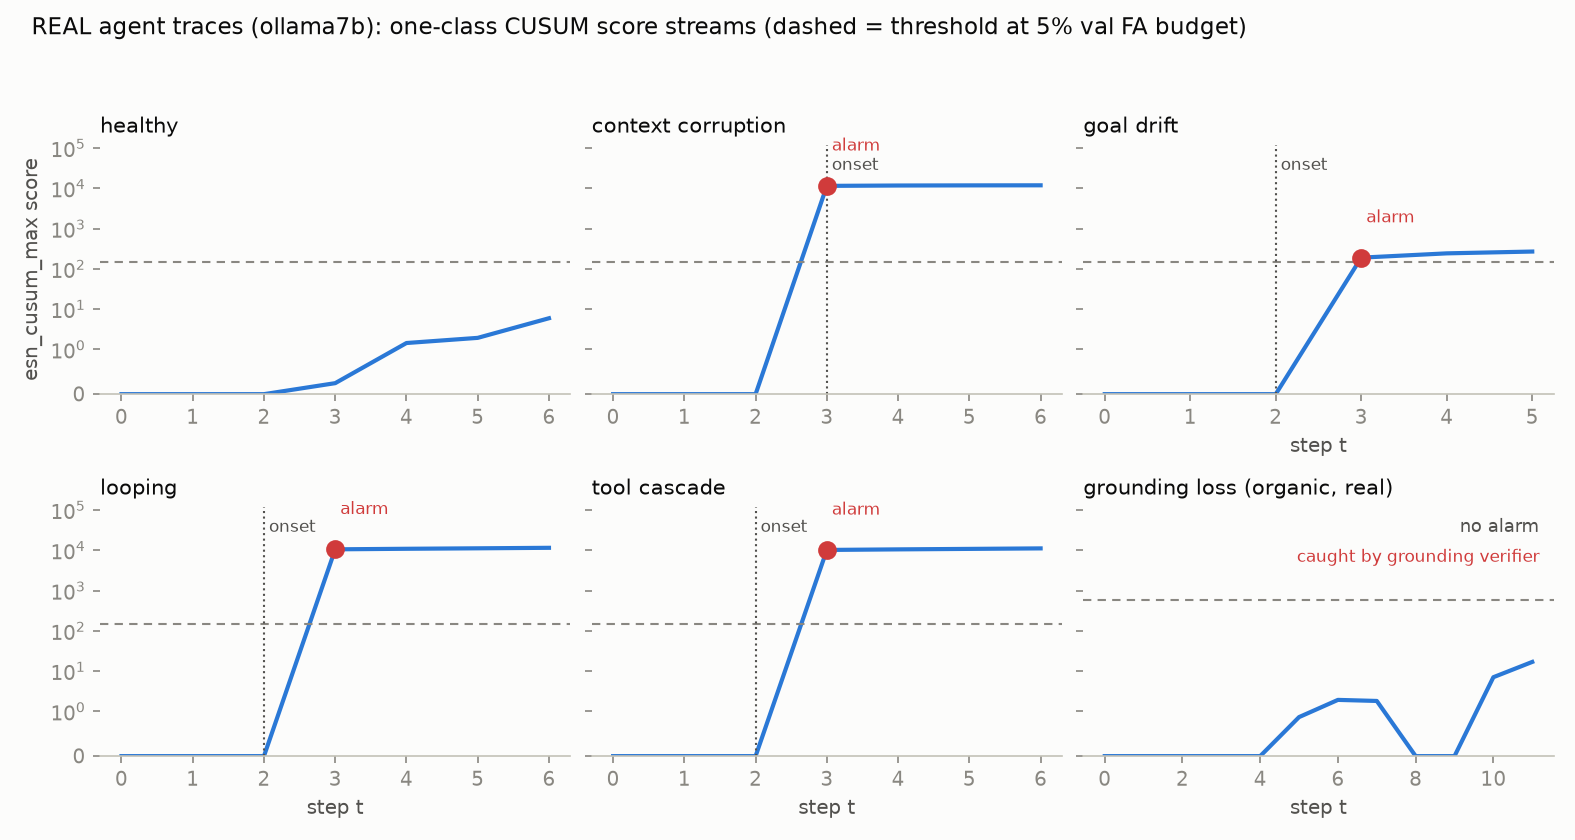
\includegraphics[width=0.94\linewidth]{fig1_score_traces_real.png}
\caption{\textbf{What the verifier sees.} One-class CUSUM streams per failure
class on real agent traces (qwen2.5:7b against real tools); dashed = threshold
at the 5\% validation budget, dotted = verified onset. Healthy stays two orders
of magnitude below the line and every injected class alarms one step after
onset. The sixth panel is different in kind: fabrication cannot be injected
into a live run, so it is a genuine organic episode --- the CUSUM stays flat,
because a fabricated figure perturbs no behavioural channel, and the class is
caught instead by the deterministic verifier of \S\ref{sec:verify}. That is the
observability boundary shown rather than asserted. The $y$ axis is symlog: the
CUSUM accumulates multiplicatively once a failure takes hold.}
\label{fig:traces}
\end{figure}

\begin{figure}[t]
\centering
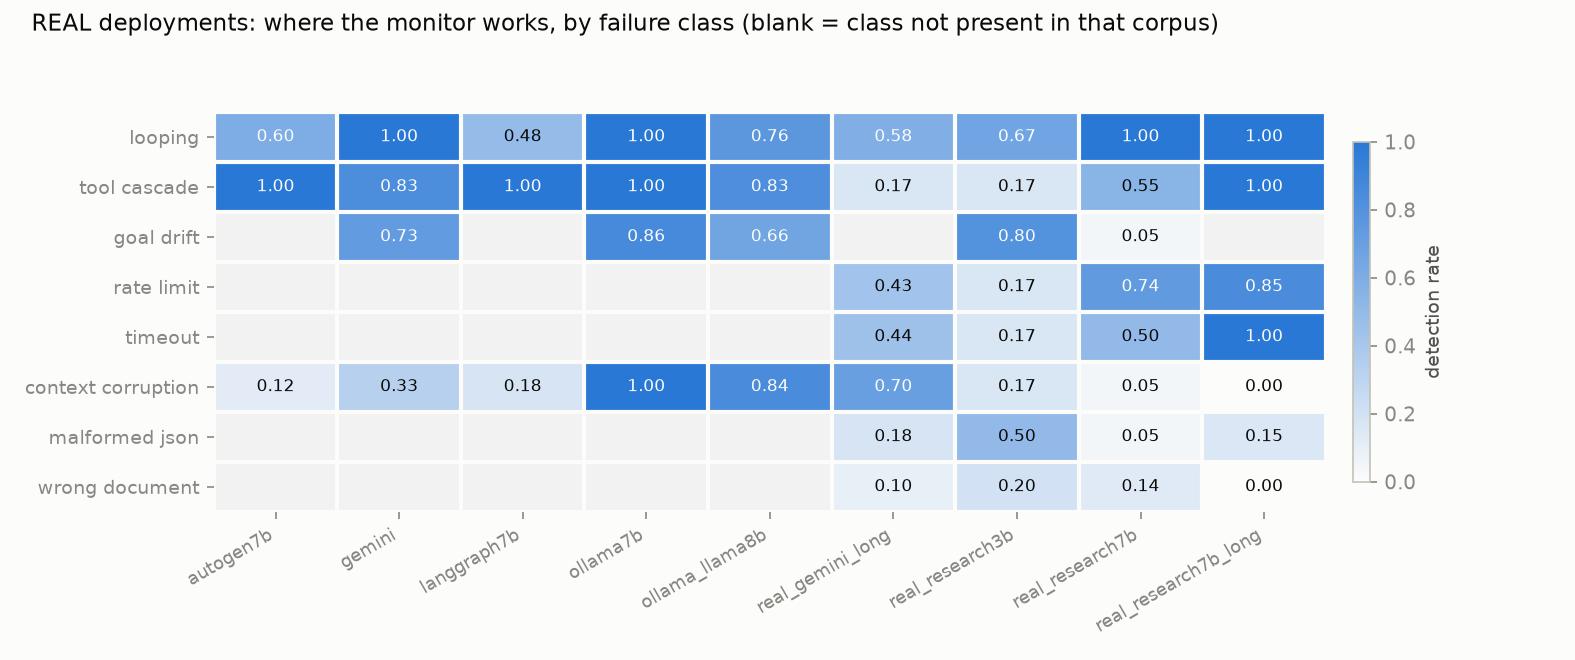
\includegraphics[width=0.96\linewidth]{fig3_class_coverage_real.png}
\caption{\textbf{Where the monitor works, by failure class}, across nine real
corpora; blank where a corpus does not contain that class, because absent and
undetected are different claims. Looping and tool cascade are caught almost
everywhere and goal drift wherever present; the weak spots are exactly the
content classes that motivate \S\ref{sec:grounding}.}
\label{fig:coverage}
\end{figure}

\section{The Horizon Law}
\label{sec:horizon}

Over 1{,}002 injected episodes the ESN\,--\,Mahalanobis detection gap is
$+0.09$ at post-onset horizon $\le3$ steps, $+0.14$ at 4--8 and $\mathbf{+0.40}$
at $\ge9$ (correlation $+0.25$). The reservoir needs post-onset steps to
integrate evidence: where it has them it wins decisively, and where it does not
its margin collapses and the memoryless distance becomes competitive. This is a
statement about \emph{regime}, and it is what makes the monitor's failures
predictable rather than mysterious.

\paragraph{The fusion buys robustness, not dominance.} A cross-fit logistic
fusion of the two parents reaches grand-mean AUROC 0.826 against 0.802 (ESN)
and 0.807 ($\Delta$-Mahalanobis), because each parent collapses on some dataset
and the fusion never does. Measured against whichever parent is better
\emph{on that dataset}, however, it is at or below it on 7 of 8 datasets in
AUROC (mean $-0.014$) and on all 8 in detection rate (mean $-0.140$).

The robustness that buys is real but conditional, and \S\ref{sec:external}
contains its counterexample: on ATBench the memoryless parent is at chance
(0.457) and drags every 50/50 blend down with it (0.438--0.463) against the ESN
alone at 0.779, while on AFTraj the same fusion is marginally ahead ($+0.015$).
Fusion protects against \emph{a} parent being weaker; it does not protect
against one being uninformative, because a 50/50 blend has no way to notice.
The hybrid is a reasonable default when the regime is unknown \emph{and} both
parents are known to carry signal --- not a general safety net, and not a
dominance result.

\section{External Validation on Corpora We Did Not Build}
\label{sec:external}

Every number above comes from corpora we collected, so none of them says
whether the benchmark is hard. We therefore ran the monitors, unchanged and
fitted on each corpus's own healthy runs, against two external benchmarks.

\paragraph{AFTraj-2K}~\cite{zhang2026agentforesight} contributes 1{,}882
multi-agent trajectories after the same $T\ge4$ filter (1{,}111 healthy, 771
failed) with a judge-annotated earliest-decisive-error step. \emph{Ranking
transfers zero-shot}: episode AUROC \textbf{0.745} on another group's agents and
frameworks, with the uncertainty channel absent entirely, against 0.802 pooled
on our own. \emph{The horizon law predicted the operating point, and held}:
detection is \textbf{0.509} on failures with $\ge9$ steps of runway against
0.170 for the memoryless baseline, but only 53 of 771 AFTraj failures have that
much room and 61\% end within three steps of onset, so pooled detection is
\textbf{0.048}. That pooled figure is the mechanism's prediction, not an excuse
offered after seeing it: \S\ref{sec:horizon} fixed the relationship on our
corpora, and AFTraj supplies a failure distribution concentrated where the
relationship says detection is impossible. A law that forecasts its own failure
region and then survives a corpus it never saw is stronger evidence than a
higher pooled number would have been.

\paragraph{ATBench}~\cite{atbench2026} contributes 604 trajectories (279 safe,
325 unsafe) labelled under a different taxonomy of risk source, failure mode and
harm. Here the monitor \emph{alarms}: AUROC \textbf{0.779} at detection
\textbf{0.311}, because ATBench's unsafe behaviour is a pattern of action --- an
over-privileged call, an unvalidated tool result --- rather than a single wrong
value. Two independent confirmations fall out. The fusion collapses to chance
(0.457 for the memoryless parent, dragging every 50/50 blend to 0.438--0.463
against the ESN's 0.779 alone), which is \S\ref{sec:horizon}'s
pooled-not-dominant finding shown on foreign data. And per failure mode the
split is sharp --- over-privileged actions 0.508 and unvalidated tool outputs
0.473 against inaccurate information \textbf{0.038} --- reproducing, on labels we
did not write, exactly the content blind spot \S\ref{sec:grounding} exists for.

For scale: an LLM auditor on AFTraj reports 66.44 Exact-F1 using a model call at
every step~\cite{zhang2026agentforesight}. We do not match that and do not claim
to; detection at a false-alarm budget is not Exact-F1. The comparison we can
make is cost: 173\,$\mu$s and no model call, against one 7B forward pass.

\section{The Judge Is a Verifier Too, and It Should Be Measured}
\label{sec:judge}

The default answer to ``who verifies the agent'' is another LLM. Escalation
analyses --- ours included --- usually \emph{stipulate} that judge's operating
point. We measured it instead. A gemini-2.5-flash judge on a labelled subset of
161 distinct prompts scores $p_{\text{detect}}=\mathbf{0.548}$ (95\% CI
0.44--0.65) and $p_{\text{false}}=\mathbf{0.052}$, against the 0.90/0.02 the
analysis assumed; both stipulated values lie outside their measured intervals.
Substituting the measured rates and re-running all five master seeds with
everything else fixed, the \emph{call saving survives} (6\% of judge-every-step
calls) but detection recovery falls from 83\% to \textbf{44\%}, supported at
\textbf{0 of 5 seeds}. We report the escalation layer's detection claim as 44\%.

The layer is still worth having, for a reason that only appears once both are
measured on the same episodes: judge and monitor fail on \emph{different}
classes (Figure~\ref{fig:complementarity}). The judge is perfect on goal drift
(21/21) and nearly blind on context corruption (0.18), where the monitor is the
reverse (1.00). That is the empirical case for escalation as a complementary
verifier rather than a more expensive approximation of the cheap one --- and a
caution against citing a stipulated judge as a baseline.

\begin{figure}[t]
\centering
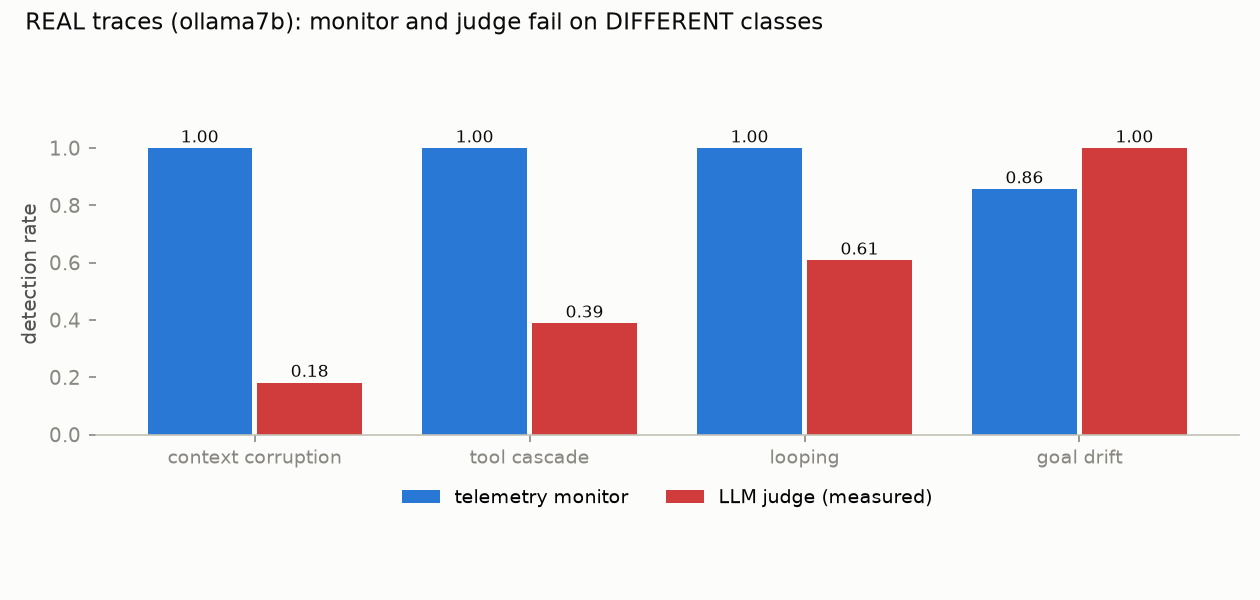
\includegraphics[width=0.82\linewidth]{fig5_judge_complementarity_real.png}
\caption{\textbf{Monitor and judge fail on different classes}, both measured on
the same real corpus. The judge is perfect on goal drift and nearly blind on
context corruption; the monitor is the reverse. Complementary verifiers, not
substitutes.}
\label{fig:complementarity}
\end{figure}

\section{The Observability Boundary and the Grounding Channel}
\label{sec:grounding}

Behavioural monitors share one blind spot: corruption that changes \emph{data}
without changing \emph{behaviour}. A wrong-but-well-formed number perturbs no
channel in \eqref{eq:features}, so no reference-free detector can reject it.
The $g$ channel adds nine causal content features --- query--result
dissimilarity, result self-consistency, JSON-prefix validity, character
anomaly, and a binary lexical-relevance flag costing 2\,$\mu$s --- which makes
query--evidence--reasoning \emph{inconsistency} observable without claiming to
observe truth. Pooled over 602 injected episodes, the content gate lifts
content-class detection $0.23\to\mathbf{0.40}$ and behavioural detection
$0.73\to\mathbf{0.80}$, gaining 37 and 25 discordant detections against zero
lost.

The boundary is real and we measured its floor: on a plausible-corruption set,
richer MiniLM embeddings leave detection at \textbf{0.00} while behavioural
AUROC falls 0.82 to 0.70, at 4.4\,ms per text and 90\,MB. The failure is
observability, not feature capacity --- which is the argument for
\S\ref{sec:verify} rather than for a bigger encoder.

\section{Deterministic Verification, and Repair}
\label{sec:verify}

The monitor needs a healthy null per deployment and spends part of a
false-alarm budget. A check needs neither. \texttt{total\_consistency}
recomputes a run's stated total from the tool results \emph{that run actually
received}; \texttt{required\_coverage} confirms every call the task requires was
made; \texttt{tool\_contract} asks whether a result matched any shape its tool
can return, and so reports when the result arrives rather than at the answer.
None reads the hidden world the task was generated from.

\begin{table}[h]
\centering
\caption{Checks against the behavioural monitor, same episodes and same
objective labels. Recall is comparable; the difference is precision.}
\label{tab:verify}
\begin{tabular}{lcc}
\toprule
 & checks & monitor \\
\midrule
failures caught, $T{=}0.2$ (served) & 60\% (\textbf{96\%} with coverage) & 54\% \\
false positives, $T{=}0.2$ & \textbf{0/63 = 0\%} & 11/63 = 17\% \\
failures caught, $T{=}0.9$ & 65\% (\textbf{96\%} with coverage) & 40\% \\
false positives, $T{=}0.9$ & \textbf{0/38 = 0\%} & 6/38 = 16\% \\
\bottomrule
\end{tabular}
\end{table}

The checks were written by inspecting failures in the serving arm, so that arm
cannot also be their test set. A further 120 episodes at disjoint task seeds
were collected afterwards and scored with the checks frozen: 54\% caught by
totals, \textbf{93\%} with coverage, and \textbf{0 of 64} false positives. A
llama3.1:8b arm on the \emph{same} task seeds, with nothing retuned, catches
\textbf{110 of 110} at \textbf{0 of 10} --- the checks transfer where the monitor
does not, because they carry no calibration. Across every labelled corpus
\texttt{tool\_contract} trips on \textbf{0 of 1825} healthy episodes and flags
46\% of context corruption, \textbf{215 of 218} within one step of onset.

\paragraph{Repair.} Each flagged episode is rolled back to its last
fact-gathering step and re-run, paired on the identical prefix and task; the
rollback is real, and success is graded by an oracle the repair prompt never
sees. Naming which check failed --- without supplying any value --- recovers
\textbf{45\%} of genuinely-wrong runs against a 16\% resampling control
($p=0.0005$), which nets task success from \textbf{52\% to 73\%} with zero
correct runs broken. Two negative results sit inside that: routing the step to
a calculator the agent already holds does \emph{not} beat retry luck
($p=0.17$), and supplying the recomputed answer buys nothing --- 26 of 55
value-bearing hints contain the correct total outright, while the value-free
rung recovers at least as much. The recovery does not come from handing over
the answer.

Coverage is partial and the shape of the gap is measured: over five injection
classes $\times$ five seeds, every behavioural alarm is followed by a repair
attempt (21 of 21), but \texttt{goal\_drift} is the only class a retry fixes (4
of 5). Where the tool layer itself is broken a retry fetches the same broken
result, and the value of the intervention is ending the episode fast --- a loop
trap exits at exactly 10 steps against 30 without the circuit breaker.

\section{Limitations}
\label{sec:limits}

Stated as measured. (1)~\textbf{No cross-deployment transfer}: the healthy null
must be collected under the exact serving distribution; transferred across a
model family the monitor sits at chance (0.527) while the same target
recalibrated reaches 0.885. (2)~\textbf{Slow goal drift} evades every per-step
surprise monitor tested; the limit is the \emph{rate} of change, not the class
--- abrupt goal changes are caught at 0.66--0.86. (3)~\textbf{Content detection
is bounded by telemetry completeness}, not by logprob access: ablating the
token-surprisal channel moves the ESN by AUROC $+0.000$. (4)~\textbf{Plausible-value
corruption} is undetectable from telemetry by construction. (5)~\textbf{Fabrication
claims are limited by base rate}: 9 of 175 organic episodes are labelled
hallucinated and only 2 are fabricated \emph{inputs}, below the pre-registered
minimum of 10, so no detection claim is made in either direction; under
provocation the grounding verifier catches 0.55 with no healthy false positives
--- specific, but half sensitive. (6)~\textbf{Scope}: mock-tool and research-loop
tasks, two local model families and one commercial API.

\section{Related Work}

\textbf{Concurrent online failure prediction.} Detecting failure during an
episode is no longer an unoccupied position. AgentForesight reframes attribution
as online auditing and releases AFTraj-2K~\cite{zhang2026agentforesight};
weakly supervised early alerting learns turn-level risk from trajectory labels
alone~\cite{baidya2026sparse}. Both use an LLM auditor. We therefore do not
claim mid-episode detection from observable telemetry as novel; what is ours is
the cost class and the boundary analysis.

\textbf{Internals versus observables.} Hidden-state probes report predicting
failure earlier than any observable-behaviour monitor~\cite{ruan2026doomed}. We
do not dispute it: with the weights, activations are richer. The premise here is
the deployment where you do not hold them --- a hosted API, a third-party agent
--- and there the choice is between telemetry and nothing.

\textbf{Runtime enforcement} intervenes during execution but requires a
specification of what unsafe means: rule sets~\cite{wang2025agentspec} or
labelled unsafe states~\cite{wang2025probguard}. Ours is label-free and
specification-free, which is why it transfers badly and needs no rule authoring.
\textbf{Post-hoc attribution} asks which step caused a failure after the fact
and finds it hard --- 14.2\% accuracy on the responsible
step~\cite{zhang2025which}; that problem is outcome-conditioned, ours is not.
\textbf{Hallucination detection} needs model access or repeated
sampling~\cite{manakul2023selfcheckgpt,farquhar2024detecting}; tool-using agents
admit the cheaper deterministic route of \S\ref{sec:verify}.

\section{Conclusion}

A cheap verifier over step telemetry covers more of the agent-failure space than
its cost suggests, and its failures are predictable rather than arbitrary: the
horizon law says where it will not fire, and held on a corpus built by another
group. Where it structurally cannot see --- a wrong-but-well-formed value ---
the answer is not a bigger encoder but a different mechanism, and a
deterministic check that recomputes the answer from the evidence the run
received is both more precise and more portable than the monitor it
supplements. We think the useful framing for agent verification is coverage:
which cheap observable verifies which failure, measured, with the gaps stated.

\bibliographystyle{plain}
\bibliography{references}

\appendix
\section{Appendix}

\subsection{Telemetry versions}

\begin{table}[h]
\centering
\small
\begin{tabular}{llp{8.4cm}}
\toprule
Version & Dims & Content \\
\midrule
v1 & 43 & $e_t$ 32-dim hash embedding; $u_t$ 4 token-surprisal aggregates;
$m_t$ action one-hot, log latency, output length, error \\
v2 & 43 & Tool results appended into step text so corrupted results reach the
semantic channel \\
v3 & 51 & 8 derived dims: cosine drift, task-anchor similarity, tool success,
retry, per-tool latency, context ratio, reasoning depth, self-consistency \\
v4 & 60 & 9 content-grounding dims: query--result dissimilarity, result
self-consistency, JSON-prefix validity, character anomaly, lexical flag \\
\bottomrule
\end{tabular}
\caption{Causal telemetry evolution. v4 costs 608\,$\mu$s/step at the adapter;
the lexical flag alone costs 2\,$\mu$s/result.}
\end{table}

\subsection{Per-dataset hybrid results}

\begin{table}[h]
\centering
\small
\begin{tabular}{lccccc}
\toprule
dataset & ESN & $\Delta$-Maha & better parent & logistic & $\Delta$ \\
\midrule
sim                  & 0.890 & 0.786 & 0.890 & 0.889 & $-0.000$ \\
autogen7b            & 0.833 & 0.774 & 0.833 & 0.777 & $-0.056$ \\
langgraph7b          & 0.828 & 0.885 & 0.885 & 0.884 & $-0.002$ \\
ollama7b             & 0.994 & 0.895 & 0.994 & 0.982 & $-0.013$ \\
real\_research3b     & 0.556 & 0.665 & 0.665 & 0.643 & $-0.022$ \\
real\_research7b     & 0.777 & 0.848 & 0.848 & 0.847 & $-0.001$ \\
real\_research7b\_long & 0.790 & 0.849 & 0.849 & 0.857 & $+0.008$ \\
gemini               & 0.749 & 0.756 & 0.756 & 0.731 & $-0.025$ \\
\midrule
grand mean           & 0.802 & 0.807 & 0.840 & 0.826 & $-0.014$ \\
\bottomrule
\end{tabular}
\caption{Episode AUROC. The fusion beats either parent's grand mean while
sitting below the per-dataset better parent on 7 of 8.}
\end{table}

\subsection{External corpora}

\begin{table}[h]
\centering
\small
\begin{tabular}{lcccc}
\toprule
corpus & monitor & AUROC & detection & FA \\
\midrule
AFTraj-2K & esn\_cusum\_max & 0.745 & 0.048 & 0.023 \\
AFTraj-2K & hybrid\_weighted50 & 0.760 & 0.047 & 0.018 \\
ATBench   & esn\_cusum\_max & 0.779 & 0.311 & 0.071 \\
ATBench   & $\Delta$-Mahalanobis & 0.457 & 0.268 & 0.161 \\
ATBench   & hybrid\_weighted50 & 0.463 & 0.277 & 0.179 \\
\bottomrule
\end{tabular}
\caption{Monitors run unchanged on two external corpora, fitted on each
corpus's own healthy runs. Neither carries token logprobs, so both run on
$e{+}m{+}x$ only.}
\end{table}

\subsection{Reproducibility}

Code, all 2{,}823 committed traces, every result table and the figures are
publicly released under a permissive licence; the URL is withheld for review.
Each headline number in this paper is tied to a named artifact by a claim
ledger that recomputes it from the committed file on every run, and a SHA-256
manifest covers every source file, trace and result so a reader can verify the
number in the text came from the file in the repository. An end-to-end
behavioural snapshot re-runs the study at a fixed seed and compares every value
against a stored baseline.

\end{document}
